\documentclass[journal]{IEEEtran}
\usepackage[spanish]{babel}
\usepackage[utf8]{inputenc}
\usepackage[T1]{fontenc}
\usepackage{amsmath,amssymb,amsfonts}
\usepackage{graphicx}
\usepackage{booktabs}
\usepackage{cite}
\usepackage{url}
\usepackage[hidelinks]{hyperref}
 
\graphicspath{{images/}}
\addto\captionsspanish{\renewcommand{\abstractname}{Abstract}}
\addto\captionsspanish{\renewcommand{\tablename}{Tabla}}
\renewcommand{\IEEEkeywordsname}{Palabras clave}
 
\begin{document}
 
\title{Esteganografía por Enmascaramiento con Eco}
 
\author{Nasser~Brown, David~Duarte y Jose~Zúñiga%
\thanks{N.Brown, D. Duarte y J. Zuñiga son estudiantes de la Maestría en Electrónica,
Escuela de Ingeniería Electrónica, curso de Procesamiento Digital de Señales
(correo electrónico: nasserbrown@estudiantec.cr; davidduarte@estudiantec.cr; je.zuniga@estudiantec.cr).}}
 
\markboth{Procesamiento Digital de Señales, Maestría en Electrónica}%
{Brown, Duarte y Zúñiga: Esteganografía por Enmascaramiento con Eco}
 
\maketitle
 
\begin{abstract}
This paper presents the design, implementation, and evaluation of the project.
A summary of the problem, the proposed method, the main results, and the
conclusions should be written here in English.
\end{abstract}
 
\begin{IEEEkeywords}
Autocorrelación del cepstro, Convolución, Enmascaramiento con eco,
Esteganografía de audio, Solapamiento y suma.
\end{IEEEkeywords}
 
% ----------------------------------------------------------------------------------------------------------------

\section{Introducción}
\IEEEPARstart{E}{n} esta sección se debe describir el problema de investigación,
la motivación del proyecto, los objetivos generales y específicos, así como el
alcance del trabajo. El ocultamiento de información mediante eco fue propuesto
originalmente en \cite{gruhl1996echo}.
 

% ----------------------------------------------------------------------------------------------------------------

\section{Marco teórico}\label{sec:teoria}

\subsection{Núcleos de eco y convolución}
Cada bit b de valor entre 0 y 1 se codifica con el sistema LTI de la ecuación~\eqref{eq:h}:
\begin{equation}\label{eq:h}
H_b(z)=1+a_b z^{-t_b},\qquad h_b(n)=\delta(n)+a_b\,\delta(n-t_b),
\end{equation}
donde $a_b$ es la amplitud y $t_b$ el retardo del eco. La elección de estos
parámetros determina el desempeño. Para retardos largos disminuyen la tasa de
transferencia, mientras que retardos cortos pueden distorsionar la señal y
dificultar la decodificación, además las amplitudes altas facilitan la decodificación,
pero el eco puede volverse perceptible \cite{gruhl1996echo}.

\subsection{Solapamiento y suma}
La señal $x(n)$ se segmenta en ventanas $v_k(n)$ de longitud $L$. Al
convolucionar una ventana con una respuesta al impulso de longitud $N=t_b+1$,
el resultado tiene longitud $L+N-1$. Si el excedente de $N-1$ muestras no se
toma en cuenta, se inducen componentes espectrales parásitas que distorsionan
el audio y corrompen los metadatos. En el solapamiento y suma, ese excedente se
suma al inicio de la siguiente ventana como describe la ecuación~\eqref{eq:ola}:
\begin{equation}\label{eq:ola}
y(n)=\sum_{k}\left(v_k*h_{b_k}\right)(n-kL).
\end{equation}


\subsection{Autocorrelación del cepstro}
El cepstro de una señal está dado por~\eqref{eq:cepstro}:
\begin{equation}\label{eq:cepstro}
c(n)=\mathcal{F}^{-1}\left\{\ln\left(\mathcal{F}\{x(n)\}\right)\right\}.
\end{equation}
Por las propiedades de la transformada de Fourier, su autocorrelación ($R_{cc}$) puede
evaluarse en el dominio espectral con~\eqref{eq:rcc}:
\begin{equation}\label{eq:rcc}
R_{cc}(n)=c(n)*c(n)=\mathcal{F}^{-1}\left\{\ln\left(\mathcal{F}\{x(n)\}\right)^2\right\}.
\end{equation}
$R_{cc}$ tiene la propiedad de destacar los retardos de los ecos, por lo que una
ventana codificada con $h_b(n)$ presenta un pico pronunciado en $n=t_b$
\cite{gruhl1996echo}.

\subsection{Métricas de desempeño}
La tasa de recuperación es la razón entre los bits decodificados correctamente y
el total de bits codificados. La tasa de transferencia es de un bit por ventana,
$f_s/L$, por lo que depende directamente del tamaño de ventana. La calidad
perceptual del audio codificado se evalúa con la evaluación perceptual de la
calidad de voz (PESQ, por sus siglas en inglés) \cite{itu2001pesq}.


% ----------------------------------------------------------------------------------------------------------------


\section{Metodología}\label{sec:sistema}
La Fig.~\ref{fig:bloques} muestra los dos subsistemas, y la
Tabla~\ref{tab:param} resume los parámetros por defecto. El audio de entrada es
un archivo de formato de audio en forma de onda (WAV, por sus siglas en inglés)
de 44.1~kHz, 16~bits y estéreo, y se procesa un solo canal (izquierdo por
defecto).

\begin{figure}[!t]
\centering
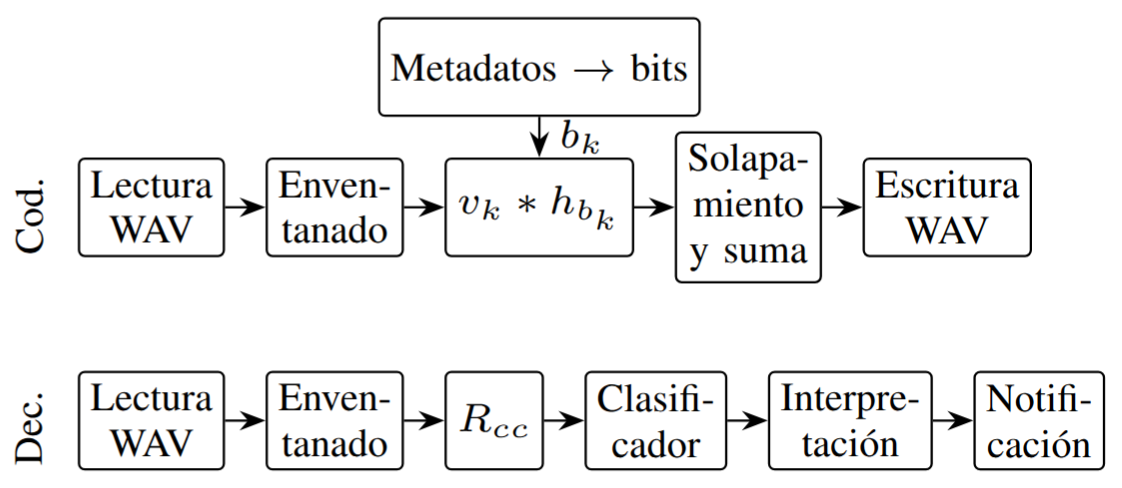
\includegraphics[width=0.75\columnwidth]{diagrama.png}
\caption{Diagrama general del sistema: codificador (arriba) y decodificador (abajo).}
\label{fig:bloques}
\end{figure}

\begin{table}[!t]
\centering
\caption{Parámetros por defecto del sistema}
\label{tab:param}
\begin{tabular}{lll}
\toprule
Parámetro & Valor & Equivalente \\
\midrule
Retardo del bit 0, $t_0$ & 1000~µs & 44 muestras \\
Retardo del bit 1, $t_1$ & 1500~µs & 66 muestras \\
Amplitudes $a_0$, $a_1$ & 40~\% & 0.4 \\
Ventana, $L=16\,t_{\max}$ & 1056 muestras & 23.9~ms \\
Tasa de transferencia, $f_s/L$ & 41.8~bit/s & --- \\
Umbral de eco, $\theta$ & 3.0 & --- \\
Ventanas sin eco de cierre, $G$ & 8 & 191~ms \\
\bottomrule
\end{tabular}
\end{table}

\subsection{Codificador}
Los retardos, dados en microsegundos, se convierten a muestras multiplicando por
$f_s$ y redondeando al entero más cercano. El tamaño de ventana depende
solo del mayor retardo, $L=16\,t_{\max}$, y es el mismo en ambos subsistemas.
Cada ventana se convoluciona explícitamente con el núcleo de su bit y se combina
con~\eqref{eq:ola}, las ventanas posteriores al mensaje se copian sin eco. La
salida se redondea y se satura al intervalo de 16~bits. 

\subsection{Decodificador}
Para cada ventana se evalúa $R_{cc}$ con~\eqref{eq:rcc} en el dominio
espectral. En la implementación se usa la magnitud del espectro y se omite la fase, 
por lo que se puede utilizar un logaritmo con números reales en lugar de complejos. 
Antes de transformar, la ventana se escala a un nivel fijo
para que la altura de $R_{cc}$ sea comparable entre ventanas de distinto
volumen, se multiplica por una ventana de Hann y se suma una constante
$\varepsilon=10^{-12}$ dentro del logaritmo para evitar $\ln 0$.

El clasificador evalúa la magnitud de $R_{cc}$ en $t_0$ y en $t_1$ y la compara
con el nivel típico de $R_{cc}$ en los retardos vecinos,
$n\in[t_{\max}/2+1,\,3t_{\max})$, mediante~\eqref{eq:z}:
\begin{equation}\label{eq:z}
z_b=\frac{R_{cc}(t_b)-\tilde\mu}{d+\varepsilon},\qquad \hat b=\arg\max_b z_b,
\end{equation}
donde $\tilde\mu$ es la mediana de $R_{cc}$ en esos retardos y $d$ la mediana
de las desviaciones absolutas respecto a $\tilde\mu$. Si $\max_b z_b<\theta$,
la ventana se clasifica como no codificada.

\subsection{Protocolo de datos y notificación}
Los metadatos se serializan como texto UTF-8 con líneas
\emph{clave}$=$\emph{valor}, y cada byte se transmite empezando por el bit más
significativo. El fin del mensaje se detecta en la primera racha de $G=8$
ventanas consecutivas sin eco. El intérprete agrupa los bits en bytes, separa
las líneas y busca cada clave en la tabla de categorías, las reconocidas se
imprimen en la salida estándar con su categoría y las desconocidas en la salida
de error con una advertencia.
 

% ----------------------------------------------------------------------------------------------------------------

\section{Resultados y Discusión}\label{sec:resultados}
Para la evaluación del sistema se usaron cuatro pistas: una pieza sintética de 30~s 
(notas armónicas con ruido de percusión), y fragmentos de rock independiente, 
piano moderno y voz narrada, convertidos a 44.1~kHz y 16~bits. En todas se 
codificaron los siete metadatos más una clave desconocida (101~bytes, 808~bits, 19.3~s).
 

% ----------------------------------------------------------------------------------------------------------------

\section{Conclusiones}
Se sintetizan los principales logros, limitaciones y propuestas de trabajo
futuro.
 

% ----------------------------------------------------------------------------------------------------------------

\bibliographystyle{IEEEtran}
\bibliography{referencias}
 
\end{document}
